\documentclass[10pt]{beamer} %
%%%BASICS
\usepackage[utf8]{inputenc}
\usepackage{csquotes}
\usepackage{multicol}
\usepackage{graphicx}
\usepackage{adjustbox}
\usepackage{textpos}
\usepackage{pgfplots}
\pgfplotsset{compat=1.15}
\usepackage[pages=some]{background}
\usepackage{minted}   %comentarios
\usepackage{caption}    % Para personalizar los títulos de floats
\usepackage{todonotes}  % Para añadir anotaciones de tareas pendientes
\presetkeys{todonotes}{inline, color=gray!30, size=\footnotesize}{}
\usepackage{easyReview} % Para añadir anotaciones de edición
\usepackage{dirtytalk}  % Para entrecomillado
\usepackage[official]{eurosym}

%\lstset{basicstyle=\footnotesize\ttfamily,breaklines=true}
%\usepackage[inline]{enumitem}
%\usepackage[inline]{enumitem}  % activar para explicar inline

\definecolor{blurple}{HTML}{7289DA}

%%%START THEME SETTINGS
\usetheme{Rochester}
\usecolortheme[named=blurple]{structure}
\usefonttheme{professionalfonts}
\setbeamertemplate{footline}[frame number]
\setbeamersize{text margin left=0.5cm,text margin right=0.5cm}
%%%END THEME SETTINGS

%\usebackgroundtemplate{
\includegraphics[width=.25\textwidth,right]{gui.png}}
\addtobeamertemplate{headline}{}{%
\begin{textblock*}{100mm}(.83\textwidth,-1.35cm)

\includegraphics[height=1.2cm]{gui.png}\vspace{220pt}
\end{textblock*}}


%%%START APA
\usepackage[spanish]{babel}
\selectlanguage{spanish}
%\usepackage[backend=biber,style=apa]{biblatex}

%%%%%%%%%%%%Titulo y autores%%%%%%%%%%%
\title[Bots de Discord]{Creación de Bots de Discord con Discord.js}
\institute[]
 {
   GUI\\
   Grupo Universitario de Informática\\
   Escuela de Ingeniería Informática, Universidad de Valladolid
 }
\author[]{Manuel de Castro Caballero} 

\date[]
 {}
\AtBeginSection[]
{
  \begin{frame}<beamer>
   \begin{multicols}{2}
     \tableofcontents[currentsection,hideothersubsections]
   \end{multicols}
  \end{frame}
}
\begin{document}

\begin{frame}
	\titlepage
\end{frame}

%------------------------------------------------------



\section{Introducción}\label{sec:intro}


\begin{frame}{Introducción}
\begin{columns}[]
\begin{column}{.5\linewidth}
	\begin{itemize}
	\item \textbf{Discord:} chat de voz y texto enfocado a videojugadores.
	\item \textbf{node.js:} \textit{runtime} de javascript con base similar a Chrome.
	\begin{itemize}
	    \item \textbf{JavaScript:} lenguaje interpretado enfocado al desarrollo de páginas web.
	\end{itemize}
	\end{itemize}
	\end{column}
	\begin{column}{.5\linewidth}

    \begin{figure}[h]
		
\includegraphics[width=.6\linewidth,]{discord.jpg}%
		\caption{Logo de discord}
		\label{fig:discord}
		\end{figure}
	
	\begin{figure}[h]
		
\includegraphics[width=.6\linewidth,]{node.png}%
		\caption{Logo de node.js}
		\label{fig:node}
		\end{figure}
\end{column}
\end{columns}
\end{frame}

\begin{frame}{JavaScript}
\begin{columns}[]
\begin{column}{.5\linewidth}
    \begin{itemize}
        \item Sintaxis relativamente similar a Java...
        \item ... no tiene nada que ver con Java.
        \item Scripting $\rightarrow$ interpretado.
        \item (Se ejecuta en el cliente.)
        \item ...
        \item No hace falta saber de antemano JavaScript para hacer un bot de Discord.
    \end{itemize}
\end{column}
\begin{column}{.5\linewidth}
    \begin{figure}
        \centering
        
\includegraphics[width=.6\linewidth]{javascript.png}
        \caption{Logo de JavaScript}
        \label{fig:jsl}
    \end{figure}
\end{column}

\end{columns}
\end{frame}

\begin{frame}{Node.js}
    \begin{itemize}
        \item Se utiliza para ejecutar JavaScript sin un navegador.
        \item Instalación: \\ \url{https://nodejs.org/}
    \end{itemize}
\end{frame}
    
\section{Creando un bot de Discord}

\begin{frame}{Discord.js}
\begin{columns}
\begin{column}{.5\linewidth}
    \begin{itemize}
        \item Módulo de \textbf{node.js} para interactuar con la API de Discord.
        \item Básicamente la opción más popular para hacer bots de Discord.
        \item Ventajas sobre otras librerías/modulos. [...]
        % \item Instalación: \\ \texttt{npm install discord.js}
        \item Documentación: \\ \url{https://discord.js.org/#/docs/main/stable/general/welcome}
    \end{itemize}
\end{column}
\begin{column}{.5\linewidth}
    \begin{figure}
        \centering
        
\includegraphics[width=0.4\linewidth]{djs.png}
        \caption{Logo de Discord.js}
        \label{fig:logo Djs}
    \end{figure}
    \vspace{-.5cm}
    \begin{figure}
        \centering
        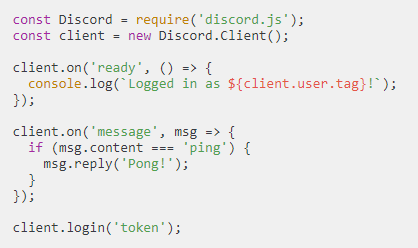
\includegraphics[width=1\linewidth]{example.png}
        \caption{Ejemplo de uso de Discord.js}
        \label{fig:Djs ex}
    \end{figure}
\end{column}
\end{columns}
\end{frame}

\begin{frame}{Registrar un bot en discord}
    \begin{itemize}
        \item (Iniciar sesión en Discord desde el navegador.)
        \item Crear una aplicación de Discord: \\ \url{https://discordapp.com/developers/applications/}
        \item Bot $\rightarrow$ Añadir Bot
        \item Profit.
        \item \textbf{Token}: Identificador del bot \textbf{en todo Discord}. \\ \textbf{IMPORTANTE} mantenerlo secreto. \vspace{.4cm}
        \item Añadir bot a un servidor (2 opciones): \\
        \begin{itemize}
            \item[--] OAuth2 $\rightarrow$ Scopes (seleccionar ``Bot'') $\rightarrow$ Acceder a la URL generada.
            \item[--] \url{https://discordapi.com/permissions.html} \\ Pegar la \textsc{client id} de nuestra aplicación $ \rightarrow $ Acceder a la URL generada.
        \end{itemize}
    \end{itemize}
\end{frame}

\begin{frame}{Creando el entorno javascript}
    \begin{itemize}
        \item (Nueva carpeta para nuestro bot.)
        \item Iniciar terminal en el directorio del bot.
        \item Entorno general: \\ \texttt{npm init}
            \begin{itemize}
                \item[--] Rellenar, o dejar los valores por defecto: nombre, versión, descripción, script de inicio, comando de prueba, repositorio git, palabras clave, autor, licencia.
                \item[--] Confirmar (yes).
            \end{itemize}
        \item Dependencias de discord.js: \\ \texttt{npm install discord.js}
        \item (Opcional) Cargador de variables de entorno: \\ \texttt{npm install dotenv} \\ (o cualquier otro módulo equivalente)
    \end{itemize}
\end{frame}

\section{Estructura básca}
\begin{frame}[fragile]{.env}
    Fichero \textbf{privado} con las \textit{variables de entorno}. No debería compartirse. (Añadir en .gitignore.)
    \begin{verbatim}
    TOKEN=[token del bot de Discord; el que hemos copiado antes.]
    PRE=[prefijo para los comandos. Suele ser "!".]
    ROL=[rol mínimo para interactuar con el bot.]
    [...]
    \end{verbatim}
\end{frame}
\begin{frame}[fragile]{index.js}
    \begin{itemize}
        \item Importar discord.js en una constante:
        \begin{minted}{javascript}
        const Discord = require("discord.js");
        \end{minted}
        \item Inicializar las variables de entorno:
        \begin{minted}{javascript}
        require("dotenv").config();
        \end{minted}
        \item Creación y registro del bot (como objeto):
        \begin{minted}{javascript}
        const bot = new Discord.Client();
        bot.login(process.env.TOKEN);
        \end{minted}
    \end{itemize}
\end{frame}
\subsection{Orientación a eventos}
\begin{frame}[fragile]{Orientación a eventos: Mensaje de bienvenida}
    Acción al iniciarse el bot, utilizando una función lambda:
    \begin{minted}{javascript}
    bot.on("ready", () => {
        console.log("Hola Discord!");
    });
    \end{minted}
\end{frame}
\begin{frame}[fragile]{Validación de comandos}
    Detectamos un mensaje; comprobamos que cumple las características de ``comando'':
    \begin{minted}{javascript}
    bot.on("message", msg => {
        // IMPORTANTE: no interactuar con bots.
        if (msg.author.bot)
            return;
        
        // Comprobar prefijo:
        if (!msg.content.startsWith(process.env.PREFIX))
            return;
        
        // Comprobar rol del autor:
        if (!msg.member.roles.find(r =>
            r.name === process.env.ROL))
            return;
            
        [...]
    });
    \end{minted}
\end{frame}
\begin{frame}[fragile]{Analizador de comandos}
    Separamos el mensaje en comando y argumentos:
    \begin{minted}{javascript}
    bot.on("message", msg => {
        [...]
        
        // Argumentos:
        let args = msg.content  // Contenido (texto) del mensaje.
            .substring(process.env.PREFIX.length) // Sin prefijo.
            .split(" ");        // Separado por espacios.
        
        // Comando:
        let cmd = args.shift()  // Primera palabra del mensaje.
                                // (Se elimina de args.)
            .toLowerCase();     // Comando en minúsculas.
            
        [...]
    });
    \end{minted}
\end{frame}
\begin{frame}[fragile]{Procesador de comandos}
    Ejecutamos el script (fichero) correspondiente al comando:
    \begin{minted}{javascript}
    bot.on("message", msg => {
        [...]
        
        try {
        
            // Actualizar el script del comando (por si acaso):
            delete require.cache[require
                .resolve(`./commands/${cmd}.js`)];
                
            // Cargar el script correspondiente:
            let cmdScript = require(`./commands/${cmd}.js`);
            cmdScript.run(bot, msg, args);
            
        } catch (e) { console.log(e.stack); }
    });
    \end{minted}
\end{frame}
\begin{frame}{Argumentos a comandos}
    \begin{itemize}
        \item \textbf{Objeto bot}, ya que es quien tiene que enviar mensajes, responder, etc...
        \item \textbf{Mensaje como objeto msg}, para acceder a sus campos como \textit{autor}, \textit{canal}, \textit{texto}...
        \item \textbf{Argumentos} del usuario para el comando, que funcionan como opciones.
    \end{itemize}
\end{frame}

\section{Encuestas en Discord}
\begin{frame}{Encuestas con reacciones}
\begin{columns}
\begin{column}{.5\linewidth}
    \begin{itemize}
        \item ¿Cómo tomáis decisiones grupales en Discord?
        \item Las encuestas con reacciones tienen numerosos inconvenientes:
        \begin{itemize}
            \item[--] Las opciones se tienen que describir en el mensaje.
            \item[--] Se puede ``votar'' a más de una opción a la vez.
            \item[--] Todas las opciones empiezan con 1 voto.
            \item[--] Se puede seguir reaccionando al mensaje con otras reacciones.
            \item[--] ...
        \end{itemize}
    \end{itemize}
\end{column}
\begin{column}{.5\linewidth}
    	\begin{figure}[h]
		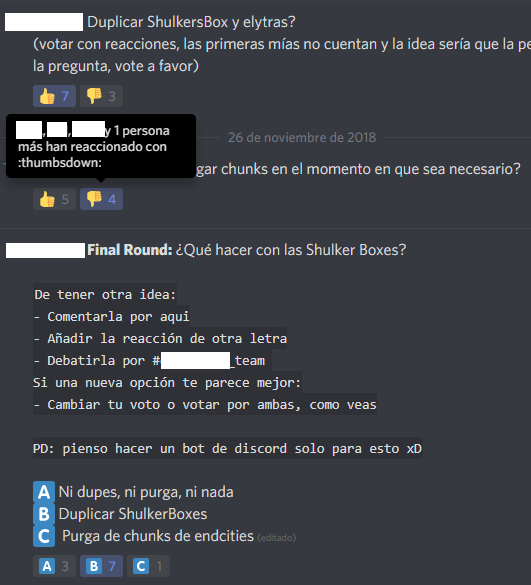
\includegraphics[width=\linewidth,]{naive_polls.png}%
		\caption{Encuestas utilizando reacciones}
		\label{fig:reacciones}
		\end{figure}
\end{column}
\end{columns}
\end{frame}
\begin{frame}{Encuestas por bots}
    \begin{itemize}
        \item Crear encuestas mediante comandos:\\\texttt{!poll [Nombre] [Opción1] [Opción2] [...]}
        \item Comandos para otras opciones: votar (\texttt{!poll vote}), cerrar (\texttt{!poll close}), ver anteriores (\texttt{!poll view}), añadir un temporizador (\texttt{!poll timer}), borrar encuestas del sistema (\texttt{!poll purge}).
        \begin{itemize}
            \item[--] Para simplificar, solo permitiremos una encuesta a la vez en el sistema (la última creada). Implementaremos \texttt{!poll}, \texttt{!poll vote} y \texttt{!poll view}.
        \end{itemize}
        \item Se utilizará ``\_'' para indicar separación de palabras en los argumentos:\\\texttt{!poll Encuesta\_de\_prueba Opción\_1 Opción\_2 Opción\_14}\\
        (El bot las reemplazará por espacios.)
        \item El resultado será un mensaje \href{https://discord.js.org/\#/docs/main/stable/class/RichEmbed}{\underline{RichEmbed}}.
    \end{itemize}
\end{frame}
\begin{frame}[fragile]{Módulo encuesta}
    \begin{itemize}
        \item Representamos las encuestas como objetos (JSON).
        \begin{itemize}
            \item[--] Las guardaremos como ficheros para poder recuperarlas.
        \end{itemize}
        \item Los votos serán listas de usuarios para cada opción (número de votos = longitud de la lista).
        \begin{itemize}
            \item[--] Para cada voto, primero se borra el usuario de todas las listas en las que esté y luego se añade a la solicitada.
            \item[--] Se mostrará el porcentaje de votos para cada opción.
        \end{itemize}
        \item Métodos:
        \begin{itemize}
            \item[--] \texttt{constructor(nombre, opciones, servidor, canal)}
            \item[--] \texttt{vote(opcion, usuario)}
            \item[--] \texttt{getTotalVotes()}
            \item[--] \texttt{save()}
            \item[--] \texttt{static fromJSON(json)}
        \end{itemize}
        \item El módulo se exporta con:
    \end{itemize}
    \begin{minted}{javascript}
    [Requires...]
    class Encuesta { [Cuerpo del módulo...] }
    module.exports = Encuesta;
    \end{minted}
\end{frame}
\begin{frame}{\texttt{constructor()}}
    Crea el objeto encuesta. Simplemente inicializa los atributos.
    \begin{itemize}
        \item \texttt{nombre}: nombre de la encuesta (se muestra en la cabecera).
        \item \texttt{opciones}: lista con todas las opciones de la encuesta. Debe tener \textbf{2 o más elementos}.
        \item \texttt{servidor}: identificador del servidor (guild) en el que se creó la encuesta, utilizado para guardar las encuestas en ficheros. Necesario si se ejecuta el mismo bot en varios servidores distintos.
        \item \texttt{canal}: identificador del canal en el que se creó la encuesta, utilizado para guardar las encuestas en ficheros. Necesario si se quiere tener encuestas distintas para cada canal (y mantener privadas las encuestas de canales privados).
    \end{itemize}
\end{frame}
\begin{frame}{\texttt{vote()}}
    Añade un voto a una opción. Debe eliminar el anterior voto del usuario, de haberlo (eliminar al usuario de las listas en las que aparezca).
    \begin{itemize}
        \item \texttt{opcion}: índice de la opción a la que añadir el voto. Debe estar \textbf{en el rango de opciones}.
        \item \texttt{usuario}: string que represente al usuario en el servidor. Debe ser \textbf{invariante y única} para cada usuario (ejemplo: nombre de usuario con discriminador: Pepito\#0420).
    \end{itemize}
\end{frame}
\begin{frame}{\texttt{getTotalVotes()}}
    Devuelve el número total de votos en la encuesta (contando todas las opciones). Utilizado para calcular el porcentaje de votos en una opción.
\end{frame}
\begin{frame}[fragile]{\texttt{save()}}
    Guarda la encuesta en un fichero JSON para poder recuperarla luego.
    \begin{minted}{javascript}
    let fs = require("fs");
    
    [...]
    
    save() {
        // Guardamos la encuesta en una carpeta
        // con el servidor por nombre:
        let dir = `./encuestas/${this.servidor}`;
        // Creamos la carpeta si no exite:
        if (!fs.existsSync(dir)) fs.mkdirSync(dir);
        
        // La encuesta se guarda con el nombre del canal:
        fs.writeFile(`${dir}/${this.canal}.json`,
            JSON.stringify(this), // String JSON del objeto.
            err => if (err) throw err);
    }
    \end{minted}
\end{frame}
\begin{frame}[fragile]{\texttt{static fromJSON()}}
    Carga una encuesta a partir de un fichero JSON.\par
    Un fichero JSON no guarda los métodos de un objeto, solo sus atributos. Hay que crear una nueva encuesta (lo que crea sus métodos), y asignarle los atributos del JSON.
    \begin{itemize}
        \item \texttt{json}: objeto JSON creado a partir del fichero de la encuesta.
    \end{itemize}
    \begin{minted}{javascript}
    static fromJSON(json) {
        // Creamos un objeto encuesta "por defecto" temporal:
        let enc = new Encuesta("", [0, 0], ".temp", ".temp");
        
        // Le asignamos el objeto JSON:
        // (Es decir, le pasamos los atributos del objeto JSON.)
        Object.assign(enc, json);
        return enc;
    }
    \end{minted}
\end{frame}
\begin{frame}{poll.js}
    Script que se ejecuta cuando el bot recibe el comando \texttt{!poll}.
    \begin{itemize}
        \item Debe importar el módulo Encuesta y \texttt{"fs"} (para abrir la encuesta del canal).
        \item Se utilizará un switch para ejecutar la opción correcta del comando.
        \item Implementará un método asíncrono \texttt{async enviar(encuesta, msg)} que enviará el RichEmbed de la encuesta.
    \end{itemize}
\end{frame}
\begin{frame}{\href{https://discord.js.org/\#/docs/main/stable/class/RichEmbed}{\underline{RichEmbed}}}
\begin{columns}
\begin{column}{.5\linewidth}
    Mensajes especiales, con un borde coloreado y cosas fancy dentro.
    \begin{itemize}
        \item \texttt{setColor(color)}: cambia el color del borde.
        \item \texttt{setTitle(titulo)}: cambia el título del embed.
        \item \texttt{addField(nombre, descripción)}: añade un campo (y su descripción) al embed; hasta un máximo de 25 campos.
        \item ... (ver \href{https://discord.js.org/\#/docs/main/stable/class/RichEmbed}{\underline{documentación}}).
    \end{itemize}
\end{column}
\begin{column}{.5\linewidth}
    	\begin{figure}[h]
		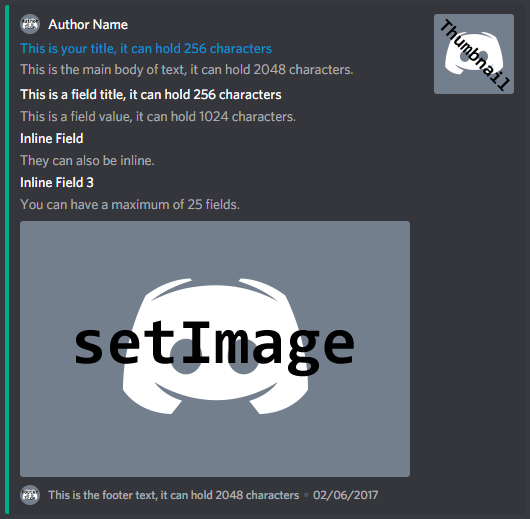
\includegraphics[width=\linewidth,]{embed.png}
		\caption{Mensaje embed de Discord}
		\label{fig:embed}
		\end{figure}
\end{column}
\end{columns}
\end{frame}
\begin{frame}{Guías para programar el bot}
\begin{itemize}
    \item Tener siempre la \href{https://discord.js.org/\#/docs/main/stable/general/welcome}{\underline{documentación}} cerca. Es muy útil.
    \item Con un \texttt{mensaje} puedes acceder a su \texttt{usuario}, su \texttt{canal} y su \texttt{guild}.
    \item Con un \texttt{canal} puedes acceder a su \texttt{guild} y a todos sus \texttt{mensajes} (como lista).
    \item Con un \texttt{guild} puedes acceder a todos sus \texttt{canales} (como lista) y a todos sus \texttt{miembros} (como lista).
    \item Con un \texttt{usuario} puedes acceder a su \texttt{canal de mensajes directos}.
    \item Con un objeto puedes acceder a todas sus propiedades básicas y de esperar (\texttt{nombre} e \texttt{id} para \texttt{usuarios}, \texttt{canales} y \texttt{guilds}, ...).
    \item \href{https://discord.js.org/\#/docs/main/stable/general/welcome}{\underline{...}}
\end{itemize}
\end{frame}
\section{Para finalizar...}
\begin{frame}{Agradecimientos}
\begin{itemize}
    \item Al \textbf{Grupo Universitario de Informática}, especialmente a \textbf{@HylianPablo}, por su inestimable ayuda y por proporcionar el material necesario para realizar el taller.
    \begin{itemize}
        \item[--] Seguidnos en Redes Sociales:
        \begin{itemize}
            \item[] Twitter: \href{https://twitter.com/GUI\_UVa}{\underline{@GUI\_UVa}}
            \item[] Instagram: \href{https://www.instagram.com/gui_uva/}{\underline{@gui\_uva}}
        \end{itemize}
    \end{itemize}
    \item A \textbf{RetroDevelopment}, porque \textst{le he copiado mucho codigo} su código me sirvió como guía a la hora de aprender a hacer bots de Discord y plantear este taller.
    \item A \textbf{todos los asistentes}, por su entusiasmo por aprender más.
\end{itemize}
\end{frame}
\begin{frame}{Contacto y dudas}
\begin{itemize}
    \item \textbf{GitHub}: \href{https://github.com/0xb01u}{\underline{0xb01u}}
    \item \textbf{Telegram}: @bomilk
    \item \textbf{Presencial}: sede del GUI. Si no estoy, preguntad por Bolu.
    \item Intentaré resolver cualquier duda que tengáis o ayudaros a seguir desarrollando vuestro bot.
\end{itemize}
\end{frame}
\begin{frame}{¿Qué nos depara el futuro?}
\begin{columns}
\begin{column}{.5\linewidth}
    \begin{figure}[h]
	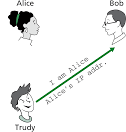
\includegraphics[width=\linewidth,]{trudy.png}
	\caption{¿Cómo podemos hacer que sólo Alice pueda enviar mensajes en su nombre?}
	\label{fig:RSA}
	\end{figure}
\end{column}
\begin{column}{.5\linewidth}
    \begin{figure}[h]
	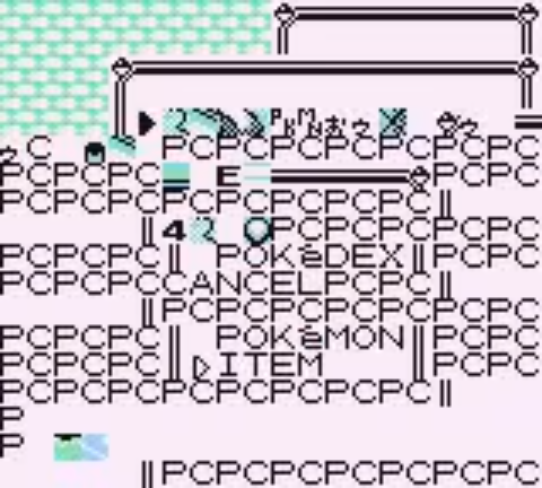
\includegraphics[width=\linewidth,]{8F.png}
	\caption{¿Cuál es este juego?}
	\label{fig:ACE}
	\end{figure}
    
\end{column}
\end{columns}
\end{frame}

\end{document}
